
%(BEGIN_QUESTION)
% Copyright 2011, Tony R. Kuphaldt, released under the Creative Commons Attribution License (v 1.0)
% This means you may do almost anything with this work of mine, so long as you give me proper credit

Sketch the wires necessary to connect a solenoid and a relay (both devices having coils rated for 120 VAC) to output channels {\tt Qx.2} and {\tt Qx.4} of a Siemens SM 322 discrete output card (model 6ES7322-1FH00-0AA0), respectively.  The internal schematic diagram of the first channel ({\tt Qx.0}) is shown as ``typical'' for all the channels, revealing how TRIACs are used to switch 120 VAC power for each discrete output channel.  Include any necessary power sources in your sketch to make the circuits functional:

$$\includegraphics[width=15.5cm]{i04246x01.eps}$$

Also, explain how the switching circuitry inside the output module functions, tracing the load current path through the module's power-switching components.

\vskip 20pt \vbox{\hrule \hbox{\strut \vrule{} {\bf Suggestions for Socratic discussion} \vrule} \hrule}

\begin{itemize}
\item{} What function does the ``SF'' LED perform, and what makes it turn on?
\end{itemize}

\underbar{file i04246}
%(END_QUESTION)





%(BEGIN_ANSWER)


%(END_ANSWER)





%(BEGIN_NOTES)

$$\includegraphics[width=15.5cm]{i04246x02.eps}$$

%INDEX% PLC, I/O: discrete I/O device wiring

%(END_NOTES)


